\newpage
\section{The Quantum Full Adder}

In this section we are going to construct, using the Qiskit SDK, a quantum circuit that implements the classic Full-Adder circuit.
We are also going to extend this circuit to compute the full addition of any $n$-qubit inputs.

\subsection{Analysing the diagram and logic of the Quantum Full-Adder}

\begin{figure}[ht]
    \centering
    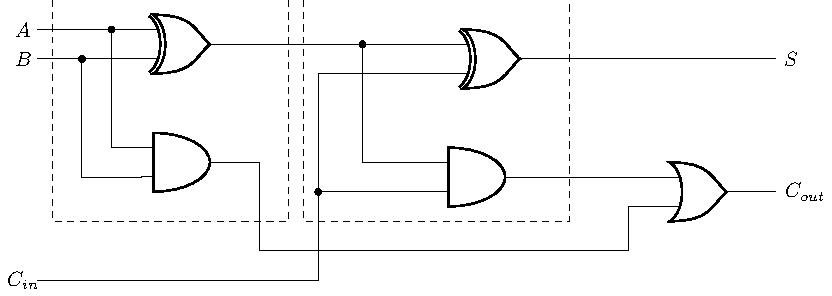
\includegraphics{images/5_Implementation/classical_fulladder_diagram.pdf}
    \caption{The classical Full-Adder circuit diagram}
\end{figure}

The Full-Adder circuit is a circuit that computes the sum $S$ and carry $C_{out}$ of two 1-bit inputs $A$ and $B$ whilist regarding a possible 1-bit
carry from some previous addition $C_{in}$. This is a much more complex circuit than the previously mentioned Half-Adder. It requires two XOR gates,
two AND gate and on OR gate. Although it seems that this circuit is bigger it can be made more simple by just considering two groups of gates. We
have indicated with two dash-lined boxes the gate-groups that are equivalent to Half-Adder circuits.

The first Half-Adder takes inputs $A$ and $B$ and produces two outputs $S_1$ and $C_1$. The second Half-Adder takes inputs $S_1$ and $C_{in}$ and produces
$S$ (which is the sum of $A + B + C_{in}$) and $C_2$. At last an OR gate is applied to $C_1$ and $C_2$ producing $C_{out}$, the carry out.

\begin{table}[ht]
    \centering
    \begin{tabular}{ccc|cc}
        $A$ & $B$ & $C_{in}$ & $S = A \oplus B \oplus C_{in}$ & $C_{out} = (A \oplus B)\cdot C_{in} + A \cdot B$ \\
        \hline
        $0$ & $0$ & $0$ & $0$ & $0$ \\
        $0$ & $1$ & $0$ & $1$ & $0$ \\
        $1$ & $0$ & $0$ & $1$ & $0$ \\
        $1$ & $1$ & $0$ & $0$ & $1$ \\
        $0$ & $0$ & $1$ & $1$ & $0$ \\
        $0$ & $1$ & $1$ & $0$ & $1$ \\
        $1$ & $0$ & $1$ & $0$ & $1$ \\
        $1$ & $1$ & $1$ & $1$ & $1$ \\
    \end{tabular}
    \caption{The truth table of the classical Full-Adder circuit}
\end{table}

We are going to implement the quantum-equivalent with the same techinque that we used to make the quantum Half-Adder circuit.
Just like the quantum Half-Adder, the AND gates need additional \say{garbage} qubits to be implemented in a quantum fashion.
Let $\ket{O}$ be the \say{garbage} qubit that will help to simulate the AND function. Also, let $\ket{A}$, $\ket{B}$ and $\ket{C_{in}}$
be the inputs.

\begin{figure}[ht]
    \centering
    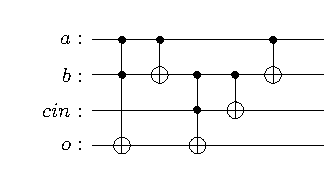
\includegraphics{images/5_Implementation/full_adder.pdf}
    \caption{The diagram of the quantum Full-Adder with slices that indicate each computational step}
\end{figure}

We are going to enumerate through all of the computational steps:
\begin{enumerate}
    \item $\ket{O} = CCNOT\ket{A,B,O} = \ket{C_1}$
    \item $\ket{B} = CNOT\ket{A,B} = \ket{S_1}$
    \item $\ket{C_1} = CCNOT\ket{S_1,C_{in},C_1} = \ket{C_{out}}$
    \item $\ket{S_1} = CNOT\ket{S_1,C_{in}} = \ket{S}$
    \item $\ket{B'} = CNOT\ket{A,S_1} = \ket{B}$
\end{enumerate}

We can see that steps 1-2 and 3-4 are gate sequences matching the behaviour of the quantum Half-Adder circuit. This means that we can replace
those gates with a gate that implements the quantum Half-Adder. Let $QHA$ be a unitary operator:

\begin{equation}
    \centering
    QHA = \begin{bmatrix}
        1 & 0 & 0 & 0 & 0 & 0 & 0 & 0  \\
         0 & 0 & 0 & 0 & 0 & 0 & 0 & 1  \\
         0 & 0 & 1 & 0 & 0 & 0 & 0 & 0  \\
         0 & 1 & 0 & 0 & 0 & 0 & 0 & 0  \\
         0 & 0 & 0 & 0 & 1 & 0 & 0 & 0  \\
         0 & 0 & 0 & 1 & 0 & 0 & 0 & 0  \\
         0 & 0 & 0 & 0 & 0 & 0 & 1 & 0  \\
         0 & 0 & 0 & 0 & 0 & 1 & 0 & 0  \\
         \end{bmatrix}
\end{equation}

Now we can edit Figure 5.5 by using the $QHA$.

\begin{figure}[ht]
    \centering
    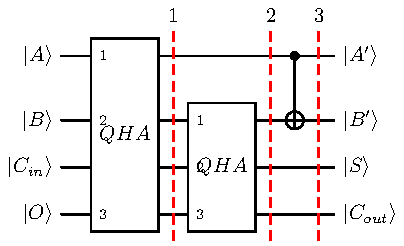
\includegraphics{images/5_Implementation/combinational_full_adder.pdf}
    \caption{The combinational quantum Full-Adder made with two Quantum Half-Adders}
\end{figure}

\subsection{The Python3 implementation}

Just like the Half-Adder implementation, we need to import the two basic classes: \\\mintinline{python3}|QuantumCircuit| and
\mintinline{python3}|QuantumRegister|. We initialize the \mintinline{python3}|circuit| object with the appropriate 1-qubit
registers $A,B,C_{in}$ and $O$.

\begin{listing}[ht]
    \begin{minted}{python3}
        from qiskit import QuantumCircuit, QuantumRegister

        a = QuantumRegister(1, name="A")
        b = QuantumRegister(1, name="B")
        cin = QuantumRegister(1, name="Cin")
        o = QuantumRegister(1, name="O")
        circuit = QuantumCircuit(a, b, cin, o)
    \end{minted}
    \caption{Initializing the quantum Full-Adder circuit}
\end{listing}

According to Figure 5.5 we have to apply five computational steps.

\begin{listing}[ht]
    \begin{minted}{python3}
        circuit.ccx(a, b, o)
        circuit.cx(a, b)
        circuit.ccx(b, cin, o)
        circuit.cx(b, cin)
        circuit.cx(a, b)
    \end{minted}
    \caption{The computations that implement the quantum Full-Adder}
\end{listing}

We can also create a custom gate to implement the Full-Adder using Half-Adders. This can be achieved my re-implementing the
quantum Half-Adder as shown in 5.1.3. and creating a new gate out of that circuit by using the \mintinline{python3}|circuit.to_gate()|
method.

\begin{listing}[ht]
    \begin{minted}{python3}
        from qiskit import QuantumCircuit, QuantumRegister
        # re-implement the half-adder circuit
        half_adder = QuantumCircuit(3)
        half_adder.ccx(0, 1, 2)
        half_adder.ccx(1, 2)
        half_adder_gate = half_adder.to_gate() # create the new gate
    \end{minted}
    \caption{Creating the Half-Adder gate}
\end{listing}

Then we can append the gate to the Full-Adder circuit by the \mintinline{python3}|circuit.append()| method. This method takes
a quantum gate as the first parameter and a list of quantum registers for the second parameter.

\begin{listing}[ht]
    \begin{minted}{python3}
        circuit.append(half_adder_gate, (a[:] + b[:] + cin[:]))
        circuit.append(half_adder_gate, (b[:] + cin[:] + o[:]))
        circuit.cx(a, b) # don't forget to restore b
    \end{minted}
    \caption{Implementating the Full-Adder with the Half-Adder gate}
\end{listing}

It is evident that Listings 5 and 7 are equivalent, they produce the exact same output. Listing 7 has the advantage of being
of a much more modular design which helps with code maintanabilty. Although it is out of the scope of this thesis we wanted
to point this design choice for the sake of transparency.

In the same spirit we can create a custom gate for the Full-Adder. Let $QFA$ be a unitary operator:

\begin{equation}
    QFA = \begin{bmatrix}
        1 & 0 & 0 & 0 & \cdots & 0 & 0 & 0  \\
         0 & 0 & 0 & 0 & \cdots & 1 & 0 & 0  \\
         0 & 0 & 0 & 0 & \cdots & 0 & 1 & 0  \\
         0 & 0 & 0 & 0 & \cdots & 0 & 0 & 0  \\
         \vdots & \vdots & \vdots & \vdots & \ddots & \vdots & \vdots & \vdots \\
         0 & 0 & 0 & 0 & \cdots & 0 & 0 & 0  \\
         0 & 0 & 0 & 0 & \cdots & 0 & 0 & 0  \\
         0 & 0 & 0 & 0 & \cdots & 0 & 0 & 0  \\
         \end{bmatrix}
\end{equation}

\begin{listing}[ht]
    \centering
    \begin{minted}{python3}
        from qiskit import QuantumCircuit, QuantumRegister
    
        a = QuantumRegister(1, name="a")
        b = QuantumRegister(1, name="b")
        cin = QuantumRegister(1, name="cin")
        o = QuantumRegister(1, name="o")
        circuit = QuantumCircuit(a, b, cin, o)

        circuit.ccx(a, b, o)
        circuit.cx(a, b)
        circuit.ccx(b, cin, o)
        circuit.cx(b, cin)
        circuit.cx(a, b)
        full_adder_gate = circuit.to_gate()
    \end{minted}
    \caption{Creating the Full-Adder gate}
\end{listing}
\newpage

We can now use the Full-Adder gate to implement much bigger quantum circuits without too much trouble. We want to point out that
this design is not particulary efficient as it uses one \say{garbage} qubit \cite{Feynman1984}. For the sake of simplicity
we are going to use this circuit as it is very straight-forward to understand.

\subsection{Extending the circuit to $n$-qubits}

The Full-Adder circuit in subsection 5.2.2 is not very useful as it can only compute the sum of 1-qubit registers. In this section
we are going to use all of the previous knowledge to create a Full-Adder circuit that can compute the sum of $n$-qubit register inputs.

By using the gate that we devised in Listing 8, we can create the Quantum Ripple Carry Adder.

For each $n$-qubits iterate over the quantum registers and apply the $QFA$ gate. We have to note that at then end of each iteration
the circuit must apply a SWAP gate on qubit $Cin_{i+1}$ and $C_{out}$. This must be applied at the end of each iteration because
$C_{out}$ stores the carry-out from the $QFA$ and it must be carried down to the next carry-in qubit for the next iteration. This
SWAP gate must not be applied at the end of the circuit because it will swap the last sum $S_{n-1}$ qubit and the $Overflow$ qubit.

\begin{listing}[ht]
    \centering
    \begin{minted}{python3}
        from qiskit import QuantumCircuit, QuantumRegister

        n = -1 # init n to a negative integer
        while n < 0:
            n = input("Input an integer (>0): ")

        a = QuantumRegister(n, name="A")
        b = QuantumRegister(n, name="B")
        cin = QuantumRegister(n, name="Cin")
        o = QuantumRegister(1, name="Cout")
        circuit = QuantumCircuit(a, b, cin, o)

        # create the full adder gate
        full_adder = QuantumCircuit(4)
        full_adder.ccx(0, 1, 3)
        full_adder.cx(0, 1)
        full_adder.ccx(1, 2, 3)
        full_adder.cx(1, 2)
        full_adder.cx(0, 1)
        full_adder_gate = full_adder.to_gate()

        # append the gate to complete the circuit logic
        for i in range(n):
            circuit.append(full_adder_gate,  (a[i], b[i], cin[i], o[:]))
            if i+1 < n:
                circuit.swap(cin[i+1], o)
    \end{minted}
    \caption{Creating the Quantum Ripple Carry Adder}
\end{listing}

\begin{figure}[!ht]
    \centering
    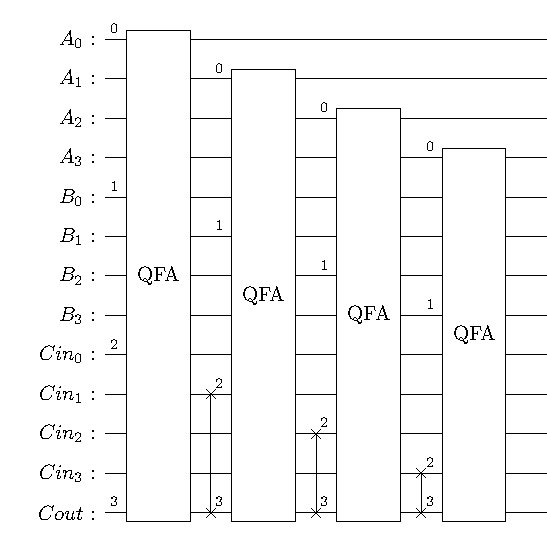
\includegraphics[height=6.5cm]{images/5_Implementation/quantum_ripple_carry_adder.pdf}
    \caption{The circuit diagram of a Quantum Ripple Carry Adder with $n=4$}
\end{figure}
